\chap{Thymio est sur une piste}\label{ch.line}

Considérez un entrepôt avec des charriots robotiques qui transportent des objets.
Il y a des lignes peintes sur le sol de l'entrepôt et le robot recoit comme instructions de suivre certaines lignes jusqu'à ce qu'il arrive à la zone de stockage de l'objet qu'il transporte.
Écrivons un programme qui permette à Thymio de suivre une ligne sur le sol.

{\raggedleft \hfill Programme: \bu{follow-line.aesl}}

Suivre une ligne sur le sol illustre le genre de difficultés rencontrées en robotique:
la ligne n'est pas forcément parfaitement droite,
de la poussière peut la recouvrir, ou de la saleté peut faire tourner une des roues du robot plus vite que l'autre.
Pour suivre une ligne malgré ces difficultés,
le robot doit utiliser un \emph{contrôleur}, qui aura pour tâche de définir la puissance à appliquer à chaque moteur en fonction des données reçues par les capteurs.

\sect{La ligne et le robot}

Pour suivre une ligne, nous allons utiliser les capteurs du sol que nous avons déjà utilisé dans le \cref{ch.moving}.
Rappelons qu'ils fonctionnent en envoyant de la lumière infrarouge (invisible pour l'oeil humain) et en mesurant la quantité de lumière renvoyée.
Si vous poser Thymio sur une couleur claire, beaucoup de lumière sera réfléchie, et donc l'événement \blksm{lots-of-light} sera déclenché.
Nous avons donc besoin d'une ligne qui déclenchera un événement quand peu de lumière sera réfléchie \blksm{little-light}.
Ceci est facile à réaliser en imprimant une bande noire, en la peignant ou en utilisant du ruban adhésif noir comme sur la \cref{fig.tape}.
La ligne doit être assez large pour que les deux capteurs de sol voient du noir quand le robot suit la ligne correctement.
Une largeur de 5 centimètres est suffisante pour que le robot suive la ligne même s'il dévie un peu.

\begin{figure}
    \subfigure[Thymio suit une ligne]
        {\label{fig.tape}
        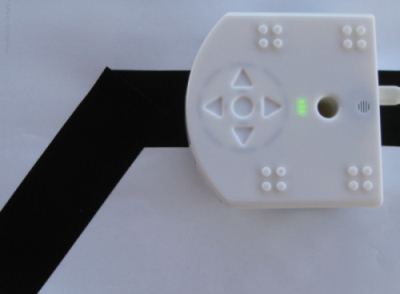
\includegraphics[height=0.35\textwidth]{blacktape}}
    \hfill
    \subfigure[Le capteur gauche est hors de la ligne,
    le capteur droite est sur la ligne. Le point rouge
    indique que le capteur gauche mesure beaucoup de lumière
    réfléchie]{
        \label{fig.one-off}
        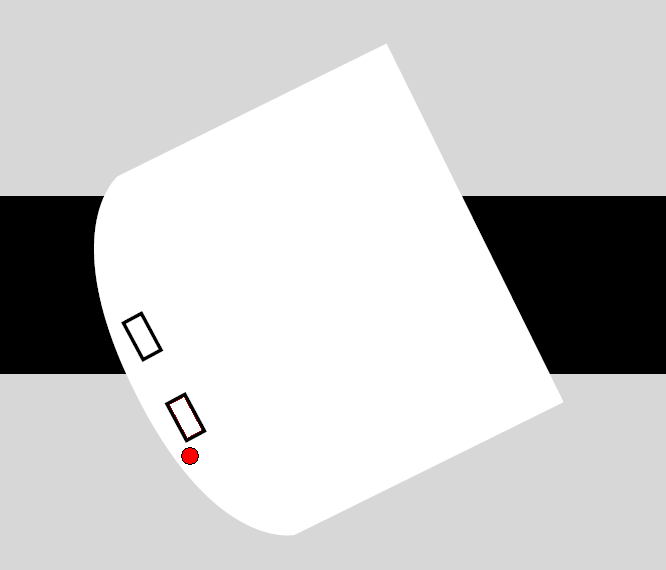
\includegraphics[height=0.35\textwidth]
        {thymio_half_on_line}}
    \caption{Thymio sur une ligne de ruban adhésif noir}
\end{figure}


Le premier pas pour faire suivre une ligne à Thymio est de le faire avancer s'il est sur la ligne (les \emph{deux} capteurs de sol détectent du foncé), et de le faire s'arrêter s'il ne se trouve pas sur la ligne (les \emph{deux} capteurs de sol détectent du clair).
Voir \cref{fig.start-stop}.

\begin{figure}
	\subfigure[Thymio s'arrête ou avance]{ \label{fig.start-stop} 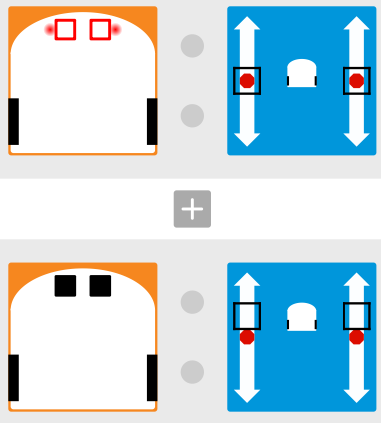
\includegraphics[width=0.4\textwidth]{line-forward}}
	\hfill
	\subfigure[Thymio corrige les déviations]{ \label{fig.follow-line} 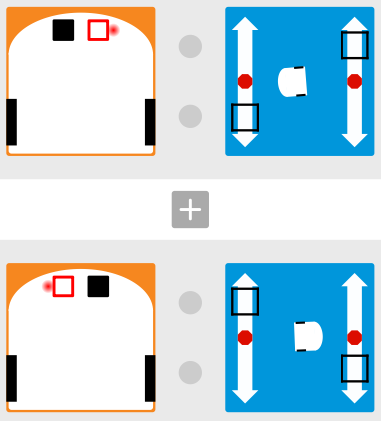
\includegraphics[width=0.4\textwidth]{line-controller}}
	\caption{Un programme pour suivre une ligne}
        \label{fig.follow-line-all}
\end{figure}

\trickbox{Assurez-vous d'avoir un câble USB assez long (disons, deux mètres) pour que le robot reste connecté même quand il bouge.
Vous trouverez des rallonges dans les magasins d'informatique.}

\sect{Votre premier contrôleur}

Le prochain pas consiste à programmer le contrôleur qui suit la ligne.
Deux paires événement-actions sont nécessaires (\cref{fig.follow-line}).

\begin{itemize}
    \item Si le robot sort de la ligne à \emph{gauche}
    \cref{fig.one-off}), le capteur \emph{gauche}
    détectera le sol alors que le capteur \emph{droite}
    continuera de détecter la ligne ;
    dans ce cas le robot doit tourner légèrement à
    \emph{droite}.

    \item Si le robot sort de la ligne à \emph{droite},
    le capteur \emph{droite} détectera le sol
    alors que le capteur \emph{gauche} continuera
    de détecter la ligne ; dans ce cas le robot
    doit tourner légèrement à \emph{gauche}.
	
\end{itemize}

\sect{Régler les paramètres}

Il est assez facile de comprendre que
si Thymio sort de la ligne à gauche,
il doit tourner à droite (\cref{fig.one-off}).
La question est plutôt: de combien doit-il tourner ?
Si la rotation est trop douce, le capteur droit pourrait aussi sortir de la ligne avant que le robot ne tourne assez ;
si au contraire le tour est trop serré, le robot pourrait sortir de la ligne de l'autre côté.
Dans tous les cas, des tours trop forts peuvent être dangereux pour le robot et ce qu'il transporte et qui risque de tomber.

Vous devrez expérimenter avec la vitesse des roues gauche et droite dans chaque bloc action moteurs
jusqu'à ce que le robot bouge de manière \emph{fiable}.
Par fiable, nous entendons que le robot peut réussir plusieurs fois l'expérience de suivi de ligne.
Comme à chaque expérience vous placez le robot sur la ligne à différentes positions et pointant dans differentes directions, il faut tester plusieurs fois pour être convaincu que le programme fonctionne.

Thymio doit-il aller vite lorsqu'il est sur la ligne ou, au contraire, lentement ?
En allant vite, vous améliorerez son efficacité pour se déplacer d'un point à un autre mais il risquera de sortir de la ligne avant de pouvoir corriger sa direction.
À l'inverse, s'il va trop lentement, personne n'achètera votre robot pour l'utiliser dans en entrepôt.
%De plus, une fois que Thymio remarque qu'il quitte la ligne, que doit-il faire ?
%S'il fait tourner un moteur dans un sens et l'autre dans le sens oppposé, vous vous assurez qu'il ne quittera pas la ligne mais ses mouvements seront très saccadés.
%S'il corrige simplement sa trajectoire en diminuant la vitesse d'une roue, il se déplacera avec fluidité, mais il risquera de quitter complètement la ligne.
%Ainsi, il faudra trouver de bons compromis.

\exercisebox{\thechapter.1}{
Thymio s'arrête complètement s'il ne détecte plus du tout la ligne.
Modifiez le programme pour qu'il tourne lentement sur lui même vers la gauche jusqu'à ce qu'il retrouve la ligne.
Essayez le sur une ligne avec un virage à gauche comme sur la \cref{fig.tape}.
Essayer d'augmenter la vitesse en avant du robot.
Que se passe-t-il lorsque le robot arrive à la fin de la ligne ?
}

\bigskip

\exercisebox{\thechapter.2}{
Modifiez le programme de l'exercice précédent pour que le robot tourne à droite quand il arrive au bout de la ligne.
Que se passe-t-il ?
\vspace{.5em}\\
Il serait bien de pouvoir se \emph{rappeller} quel capteur était le dernier à perdre le contact avec la ligne afin de faire tourner le robot dans la bonne direction pour retrouver la ligne.
Dans le \cref{ch.states}, nous apprendrons à Thymio à se rappeler ces informations.
}

\bigskip 

\exercisebox{\thechapter.3}{
Jouez avec différentes formes de parcours :
\begin{itemize}[noitemsep,nosep,leftmargin=*]
\item Des virages doux
\item Des virages serrés
\item Des zig-zag
\item Des lignes plus larges
\item Des lignes plus étroites
\end{itemize}
Faites la course avec vos amis :
Quel robot suit le plus de lignes différentes avec succès ?
Pour chaque ligne, quel robot la suit dans le moins de temps ?
}

\bigskip

\exercisebox{\thechapter.4}{
Discutez les effets que les modifications suivantes au Thymio auraient sur les capacités du robot à suivre une ligne :
\begin{itemize}[noitemsep,nosep,leftmargin=*]
\item L'événement de lecture des capteurs de sol devient plus ou moins fréquent.
\item Les capteurs sont plus éloignés ou proche l'un de l'autre.
\item Il y a plus que deux capteurs de sol sous le robot.
\end{itemize}
}

% TODO
